% version 1.00	Auteur Mathieu Medici

\documentclass[asi]{picInsa}
\usepackage{pdfpages}

% \input{commandes}

\usepackage{vocabulaireUnipik}

\definecolor{gris}{gray}{0.75}% utilisé dans les annexes A B et C
\definecolor{gris2}{gray}{0.85}% utilisé dans les annexes A B et C

\titreGeneral{\pgc}
\sousTitreGeneral{\nomEquipe}
\titreAcronyme{\pgcCourt}
\version{v1.00}
\referenceVersion{\pgcCourt\_Q\_\nomEquipe\_\versionPrive}
\titreDetaille{\pgcCourt\_Q\_\nomEquipe\_\versionPrive}
\auteurs{\Mathieu{}}
\destinataires{\nomApprobateur{}, \nomTuteurQualite, \nomEquipe, \nomPIC}
\resume{Le présent document contient la présentation du système de gestion
des configurations pour \nomEquipe.}
\natureDerniereModification{Création}
\motsCles{\pgcCourt{}, référentiel, nommage}
\modeDiffusionControle{}

\newcommand{\elementRDF}[1]{\NoAutoSpaceBeforeFDP{#1}}

%opening

%Ces deux lignes empèche LaTeX de numéroter les chapitres qui sont inexistant dans le PQ
%makeatletter\@addtoreset{section}{part}\makeatother
%renewcommand{\thesection}{\arabic{section}}

\begin{document}
 \couverture{}
 \informationsGenerales{}
  % version 1.00, date 29/02/16, auteur Michel Cressant
\begin{pagesService}
	\begin{historique}
		% nouvelles versions à rajouter AU-DESSUS en recopiant les lignes suivantes et en les modifiant :
		\unHistorique{1.00}{02/02/2016}{\Michel}{Création}{Toutes}

	\end{historique}

%        \begin{suiviDiffusions}
%
%            % On place ici les diffusions
%        	\unSuivi{1.00}{}{\nomEquipe{}}
%          
%          
%        \end{suiviDiffusions}

%%Signataires
        \begin{signatures}
	   \uneSignature{Vérificateur}{\RRS}{\Matthieu{}}{17/03/2016}{PGPic}
       \uneSignature{Validateur}{\CP{}}{\Sergi}{}{PGPic}
        \end{signatures}
	
	

	
	
\end{pagesService}

 \tableofcontents
 
 \chapter*{Introduction}
 % version 1.01 Date 24/03/2016	Auteur Mathieu Medici

\section*{Objet}
L'objectif de ce document est de présenter les principes et les procédures nécessaires à la mise en œuvre de la gestion des configurations prévue par la norme \isoNeufMilleUn.

\section*{Définition}

Le présent document établit les règles et la structure de la gestion des configurations qui doivent être suivies pendant toute la durée du \picCourt. Il contient :
\begin{itemize}
\item les règles de nommage;
\item la description des différents référentiels;
\item les règles spécifiques de \nomEquipe{};
\item la description de l'administration des configurations;
\item la description de la maîtrise des documents;
\item la description de la maîtrise des enregistrements;
\item les règles d'archivage.
\end{itemize}


 
 \chapter{Règles de nommage}
 \label{chap regle nommage}
 % version 2.00 Date 02/05/2016	Auteur Mathieu Medici
% version 1.01 Date 31/03/2016	Auteur Mathieu Medici

Dans le but d'identifier clairement et de manière unique les éléments de configuration du \picCourt{}, il est nécessaire de spécifier des règles de nommage. Chaque élément inclu dans un référentiel doit respecter la règle de nommage qui lui convient.\\

L'ensemble des fichiers suit le modèle suivant :
\begin{center}
  \verb+<Type>_<Referentiel>_Unipik_<Suffixe>+
\end{center}
On utilisera des abréviations pour chaque élément (Type, Référentiel et Suffixe).\\
Exemple de nommage: \verb+PGC_Q_Unipik_v1.00+\\
Exemple de stockage : \verb+pic_unicef/qualite/GC/PGC/+ 


\section{Nom du \picCourt{}}
Ce champ indique l'appartenance du document au \PICCourt{} peu importe sa provenance
 (PIC, client, département \ASI{}, etc). Il a pour valeur \textbf{\nomEquipe}.

\section{Référentiels}

Tous les éléments réalisés au cours du PIC appartiennent à l'un des 5 référentiels suivants : Développement, Livraison, Qualité, Ressources et Spécifications.
\begin{table}[H]
\centering
	\begin{tabularx}{11cm}{|X|c|X|}
	\hline
	\rowcolor[gray]{0.85} Référentiels & Abréviations & Noms des dossiers sous \git{} \\
	\hline
	Développement & D & developpement\\
	\hline
	Livraison & L & livraison\\
	\hline
	Qualité & Q & qualite\\
	\hline	
	Ressources & R & ressources\\
	\hline 
	Spécifications & S & specifications\\ 
	\hline
	\end{tabularx}
\caption{Abréviations associées à chaque type}
\label{Référentiel}
\end{table}

\section{Types}
Chaque document est défini par un type et sera stocké dans le dossier de même nom. Chaque type est associé à zéro, un ou deux suffixes. Voici l'ensemble des documents associé pour chacun à son type et ses suffixes:

\begin{longtable}{|p{12cm}|c|c|}
    \hline
    \rowcolor[gray]{0.85} Documents et Enregistrements & Type & Suffixe 			\endfirsthead
    \hline	
    \rowcolor[gray]{0.85} Documents et Enregistrements & Type & Suffixe \endhead
    \hline
    \multicolumn{3}{|c|}{\textbf{\bsc{suite ...}}}\endfoot
    \hline
    \endlastfoot
    \hline
    \multicolumn{3}{|c|}{\textbf{\bsc{Référentiel Qualité}}}\\
    \hline
    Dossier de Suivi de la Qualité & DSQ & -\\
    \hline
    	\hspace{1cm} Faits Techniques & FT & -\\
    	\hline   
    	\hspace{2cm} Commission de Traitement des Faits Techniques & CTFT & n,d\\
    	\hline
    	\hspace{2cm} Fiche de Fait Technique & FFT & c,n,d\\
    	\hline
    	\hspace{2cm} Fiche d'Ordre de Correction & FOC & n,d\\
    \hline
    \hspace{1cm} Fiche de Compétences & FC & p,v\\
    \hline
    \hspace{1cm} Fiche de Formation & FF & c\\
    \hline
    \hspace{2cm} Fiche Récapitulative de Cours & FRC & c\\    
    \hline
    \hspace{1cm} Fiche de Rôle & FR & r,v\\
    \hline
    \hspace{1cm} Organigramme Fonctionnel & OF & v\\
    \hline
    \hspace{1cm} Plan de Formation & PF & v\\
    \hline
    \hspace{1cm} Questionnaire de Satisfaction & QS & -\\
    \hline
    \hspace{2cm} Questionnaire de Satisfaction Client & QSC & d\\
    \hline
    \hspace{2cm} Questionnaire de Satisfaction Élève & QSE & d\\
    \hline
    \hspace{2cm} Questionnaire de Satisfaction Service Support & QSSS & d\\
    \hline
    \hspace{2cm} Questionnaire de Satisfaction Tuteur & QST & d\\    
    \hline
    \hspace{1cm} Rapport d'Audit Interne & RAI & d\\  
    \hline
    \hspace{1cm} Rapport d'Inspection Technique & RIT & d\\
    \hline
    \hspace{1cm} Tableau de Bord & TB & s\\
    \hline
    Gestion de Projet & GP & -\\
    \hline
    \hspace{1cm} Fiche de Suivi & FS & p\\
    \hline
    \hspace{1cm} Planification Projet & PP & s\\    
    \hline
    \hspace{1cm} Compte-Rendu & CR & -\\
    \hline
    \hspace{2cm} Compte-Rendu de réunion Client & CRC & d\\
    \hline
    \hspace{2cm} Compte-Rendu de réunion Exceptionnelle & CRE & d\\
    \hline
    \hspace{2cm} Compte-Rendu de réunion Interne & CRI & d\\
    \hline
    \hspace{2cm} Compte-Rendu de réunion Inter-PIC & CRIP & d\\
    \hline
    \hspace{2cm} Compte-Rendu de réunion de Fait Technique & CRFT & d\\
    \hline
    \hspace{2cm} Compte-Rendu de réunion Tuteur Pédagogique & CRTP & d\\
    \hline
    \hspace{2cm} Compte-Rendu de réunion Tuteur Qualité & CRTQ & d\\
    \hline
    \hspace{1cm} Emails & mails & -\\
    \hline
    \hspace{2cm} Mail du Client & MC & d,c\\
    \hline
    \hspace{2cm} Mail du Directeur Qualité & MDQ & d,c\\
    \hline
    \hspace{2cm} Mail de l'Equipe & ME & d,c\\
    \hline
    \hspace{2cm} Mail de Livraison & ML & d,c\\
    \hline
    \hspace{2cm} Mail de l'Unité P3 & MP3 & d,c\\
    \hline
    \hspace{2cm} Mail du Tuteur Communication & MTC & d,c\\
    \hline
    \hspace{2cm} Mail du Tuteur Pédagogique & MTP & d,c\\
    \hline
    \hspace{2cm} Mail du Tuteur Qualité & MTQ & d,c\\
    \hline
    \hspace{1cm} Procès-Verbal & PV & -\\
    \hline
    \hspace{2cm} Revue Formelle de Démarrage & RFD & -\\
    \hline
    \hspace{3cm} Procès-Verbal de Démarrage & PVD & d\\
    \hline
    \hspace{2cm} Revue Formelle de Fin de Phase de Conception Préliminaire & RFFPCP & -\\
    \hline
    \hspace{3cm} Procès-Verbal de Fin de Phase de Conception Préliminaire & PVFPCP & d\\
    \hline
    \hspace{2cm} Revue Formelle de Fin de Phase d'Intégration & RFFPI & -\\
    \hline
    \hspace{3cm} Procès-Verbal de Fin de Phase d'Intégration & PVFPI & d\\
    \hline
    \hspace{2cm} Revue Formelle de Fin de Phase de Spécifications & RFFPS & -\\
    \hline
    \hspace{3cm} Procès-Verbal de Document de Spécifications Externes & PVDSE & d\\
    \hline
    \hspace{3cm} Procès-Verbal de Document de Spécifications Internes & PVDSI & d\\
    \hline
    \hspace{3cm} Procès-Verbal de Fin de Phase de Spécifications & PVFPS & d\\
    \hline
    \hspace{3cm} Procès-Verbal de Plan de Tests de Validation & PVPTV & d\\
    \hline
    \hspace{2cm} Revue Formelle de Recettes & RFR & -\\
    \hline
    \hspace{3cm} Procès-Verbal de Recettes & PVR & d\\
    \hline
    Gestion des Configurations & GC & -\\
    \hline
    \hspace{1cm} Etat de Configuration & EC & d,c\\
     \hline
    \hspace{1cm} Fiche d'Etat des Données Client & FEDC & aucun\\   
    \hline
    \hspace{1cm} Plan de Gestion des Configurations & PGC & v\\
    \hline
    Portefeuille des Risques et Opportunités & PRO & -\\
    \hline
    \hspace{1cm} Fiche De Risque & FDR & n\\
    \hline
    \hspace{1cm} Fiche D'Opportunité & FDO & n\\
    \hline
    Plan Qualité & PQ & v\\
    \hline
 \multicolumn{3}{|c|}{\textbf{\bsc{Référentiel Spécifications}}}\\
    \hline
    Document de Spécifications Externes & DSE & v\\
    \hline
    Document De Spécifications Internes & DSI & v\\
    \hline
    Plan de Tests de Validation & PTV & v\\
    \hline
 \multicolumn{3}{|c|}{\textbf{\bsc{Référentiel Développement}}}\\
    \hline
    Dossier d'Audit de Code & DAC & d\\
    \hline
    Implémentation & implementation & -\\
    \hline
    LotX & lotX & -\\
    \hline
    \hspace{1cm} \CDR & CDR & l, v\\
    \hline
    \hspace{1cm} Dossier de Conception Détaillée & DCD & l\\
    \hline
    \hspace{1cm} Dossier de Conception Préliminaire & DCP & l\\
    \hline    
    \hspace{1cm} Dossier de Tests & DT & -\\
    \hline
    \hspace{2cm} Dossier de Tests d'Intégration & DTI & l \\
    \hline
    \hspace{3cm} Journal de Tests d'Intégration & JTI & l \\ 
    \hline
    \hspace{3cm} Plan de Tests d'Intégration & PTI & l \\
    \hline
    \hspace{2cm} Dossier de Tests Unitaires & DTU & l \\
    \hline
    \hspace{3cm} Journal de Tests Unitaires & JTU & l \\
    \hline
    \hspace{3cm} Plan de Tests Unitaires & PTU & l \\
    \hline
    \hspace{1cm} Guide Utilisateur & GU & l\\
    \hline
    \hspace{1cm} Procédure d'Installation & PI & l\\
    \hline
 \multicolumn{3}{|c|}{\textbf{\bsc{Référentiel Livraison}}}\\
    \hline   
    Lots & lots & -\\
    \hline
    \hspace{1cm} Lot numéro X & lotX & d\\
    \hline
    Réunion Bilan & RB & -\\
    \hline
    \hspace{1cm} Réunion Bilan \CP & RBCP & -\\
    \hline
    \hspace{2cm} Document de debriefing & debriefing & d,r\\
    \hline 
    \hspace{2cm} Poster du Pic & poster & d,r\\
    \hline     
    \hspace{2cm} Résumé du Pic & resumePic & d,r\\
    \hline 
    \hspace{2cm} Résumé pour le diplôme & resumeDiplome & d,r\\
    \hline 
    \hspace{2cm} Document pour la communication & docCom & d,r\\
    \hline      
    \hspace{2cm} Support Présentation pour le Debriefing & SPD & d,r\\   
    \hline            
    \hspace{1cm} Réunion Bilan \RQ & RBRQ & -\\
    \hline    
    \hspace{2cm} Document de debriefing & debriefing & d,r\\    
    \hline
    \hspace{2cm} Questions pour l'Evaluation de la DGQ & QEDGQ & d,r\\   
    \hline   
    \hspace{2cm} Support Présentation pour le Debriefing & SPD & d,r\\   
    \hline       
    Revues & revues & -\\
    \hline
    \hspace{1cm} Revue numéro X & revueX & -\\
    \hline
    \hspace{2cm} Support Présentation & SP & n\\
    \hline
  \caption{Formalisme des différents Types}
  \label{Formalisme Types}  
\end{longtable}

\section{Suffixes}

Lors du nommage nous utilisons des suffixes adaptés en fonction du type de document. Un document peut avoir plusieurs suffixes, dans ce cas ils sont séparés par un "$\_$". La présence de chaque suffixe demandé est obligatoire et dois respecter l'ordre indiqué. Les suffixes possibles sont les suivants : 

	\begin{table}[H]
		\centering
		\begin{tabularx}{10cm}{|X|c|c|}
		\hline
		\rowcolor[gray]{0.85} Suffixe & Abréviation & Format\\
		\hline
		Date & d & dAA-MM-JJ\\
		\hline
		Version & v & vX.YY\\
		\hline
		Lot & l & lX\\		
		\hline
		Numéro & n & nXXX\\
		\hline
		Semaine & s & sXX\\
		\hline
		Rôle & r & rRole\\
		\hline
		Personne & p & pInitiales\\
		\hline
		Commentaire & c & cCommentaire\\
		\hline
		\end{tabularx}
	\caption{Abréviations associées à chaque suffixe}
	\label{Suffixes}
	\end{table}
	


\subsection{Suffixe Date}
\label{suffixe_date}

Le suffixe \verb+Date+ suit le format \textbf{AA-MM-JJ}, AA pour l'année, MM pour le mois et JJ pour le jour. Ce format permet de classer les documents par ordre chronologique.\\

Exemple : \verb+d16-01-27+

\subsection{Suffixe Version}
\label{suffixe_version}
Le suffixe \verb+Version+ suit le format \textbf{vX.YY}. La gestion des versions et des révisions n'étant pas la même selon si le document doit être approuvé ou non, nous allons séparer la convention du suffixe \verb+Version+ en deux parties. \\

\paragraph{Cas des documents avec approbation\\}

Dans le cas des documents à approuver (par exemple PQ ou PGC), X est le numéro d'approbation et commence à 0, YY est le numéro de correction et commence à 00. Lorsqu'un document est approuvé, le numéro d'approbation est incrémenté et le numéro de correction revient à 00. Lorsqu'un document est corrigé suite à une demande de correction, le numéro de correction est incrémenté.

Pour plus de clarté, voici le mode de fonctionnement étape par étape : 
\begin{itemize}
\item[$\rightarrow$] Création d'un document en v0.00;
\item[$\rightarrow$] Envoi du document en v0.00 pour approbation;
\item[$\rightarrow$] Demande de correction sur le document en v0.00;
\item[$\rightarrow$] Correction du document en v0.01;
\item[$\rightarrow$] Envoi du document en v0.01 pour approbation;
\item[$\rightarrow$] ...;
\item[$\rightarrow$] Approbation du document en v1.00 et diffusion obligatoire du document en version v1.00;
\item[$\rightarrow$] Envoi du document en v1.01 pour approbation;
\item[$\rightarrow$] Demande de correction sur le document en v1.01;
\item[$\rightarrow$] Correction du document en v1.02;
\item[$\rightarrow$] Envoi du document en v1.02 pour approbation;
\item[$\rightarrow$] ...;
\item[$\rightarrow$] Approbation du document en v2.00 et diffusion obligatoire du document en version v2.00;
\end{itemize}

\paragraph{Cas des documents sans approbation\\}

Dans le cas des documents n'ayant pas besoin d'être approuvés (par exemple DSI), X est le numéro de version classique et commence à 1, YY n'est pas utilisé.

Pour plus de clarté, voici le mode de fonctionnement étape par étape :
\begin{itemize}
\item[$\rightarrow$] Création du document en v1.00;
\item[$\rightarrow$] Modification du document en v2.00;
\item[$\rightarrow$] Modification du document en v3.00;
\item[$\rightarrow$] ...
\end{itemize}


\subsection{Suffixe Lot}
\label{suffixe_lot}


Le suffixe \verb+Lot+ suit le format \textbf{lX}. X correspond au numéro du lot.\\

Exemple : \verb+l1+\\


\subsection{Suffixe Numéro}
\label{suffixe_numero}

Le suffixe \verb+Numéro+ suit le format \textbf{nXXX}. XXX est un nombre entier compris entre 001 et 999. Il commence à la valeur 001 et est incrémenté à chaque nouveau document.\\

Exemple : \verb+n042+\\

Remarque : Petit cas particulier pour les numéros des documents situés dans un dossier \verb+revuesX+. Le suffixe numéro correspond dans ce cas précis au numéro de la revue et suit le format \textbf{vX} avec X le numéro de la revue.\\


Exemple : \verb+n1+\\

\subsection{Suffixe Semaine}
\label{suffixe_semaine}

Le suffixe \verb+Semaine+ suit le format \textbf{sXX}. XX correspond au numéro de la semaine en cours, la première semaine du PIC étant 01. Seules les semaines comportant au moins un jour ouvré sont numérotées.\\

Exemple : \verb+s09+

\subsection{Suffixe Rôle}
\label{suffixe_role}

Le suffixe \verb+Rôle+ suit le format \textbf{rRole} où Role correspond au rôle concerné par le document. Les valeurs possibles pour Role sont : 
\begin{itemize}
\item CP :  \CP;
\item CPA : \CPA;
\item RQ : \RQ;
\item RQA : \RQA;
\item RGC : \RGC;
\item RRS : \RRS;
\item RS : \RS;
\item RD : \RD;
\item D : \D;
\item PR : \PDR.\\
\end{itemize}

Exemple : \verb+rCP+

\subsection{Suffixe Personne}
\label{suffixe_personne}

Le suffixe \verb+Personne+ suit le format \textbf{pInitiales} où Initiales correspond aux initiales de la personne concernée par le document. Dans le cas où plusieurs personnes sont concernées le suffixe aura le format \textbf{pInitiales1-Initiales2}. Les initiaux possibles sont les suivants :
\begin{table}[H]
	\centering
	\begin{tabularx}{8cm}{|X|c|}
	\hline
	\rowcolor[gray]{0.85} Personnes & Initiales\\
    \hline
    \Francois & FD \\
	\hline
	\Florian & FL \\
	\hline
	\Julie & JP \\
	\hline
	\Juliana & JR \\
	\hline
	\Kafui & KA \\
	\hline
	\Melissa & MB \\
	\hline
	\Michel & MC \\
	\hline
	\Mathieu & MM \\
	\hline
	\Matthieu & MMB \\
	\hline
	\Pierre & PP \\
	\hline
	\Sergi & SC \\
	\hline
	\end{tabularx}
	\caption{Initiales associées à chaque personne}
	\label{Initiales}
\end{table}

Exemple : \verb+pFL+

\subsection{Suffixe Commentaire}
\label{suffixe_commentaire}

Le suffixe \verb+Commentaire+ suit le format \textbf{cCommentaire} où Commentaire a une valeur bien précise selon le type de document. Pour \nomEquipe, il y a cinq documents différents ayant un suffixe \verb+commentaire+, voici leurs valeurs associées :
\begin{itemize}
\item Fiche de Formation (FF) : sujet de la formation;\\
 Exemple : \verb+cLaTeX+
 \item Fiche Récapitulative de Cours (FRC) : sujet du cours;\\
 Exemple : \verb+cLaTeX+
\item emails (MC, MDQ, ML, MP3, MTC, MTP, MTQ) : sujet de l'email;\\
 Exemple : \verb+cdatesRevues+
\item Fiche de Fait Technique (FFT) : peut prendre deux valeurs, \verb+RC+ si c'est un fait technique suite à une réclamation client, \verb+autre+ sinon;\\
 Exemple : \verb+cRC+
\item Etat de Configuration (EC) : voir la partie \ref{EC}.
\end{itemize}


 \chapter{Structure des référentiels}
 \label{chap struc ref}
  % version 1.01 Date 08/03/2016	Auteur Mathieu Medici

Les référentiels sont stockés selon la structure suivante : 

\begin{figure}[ht]
         \begin{center}
         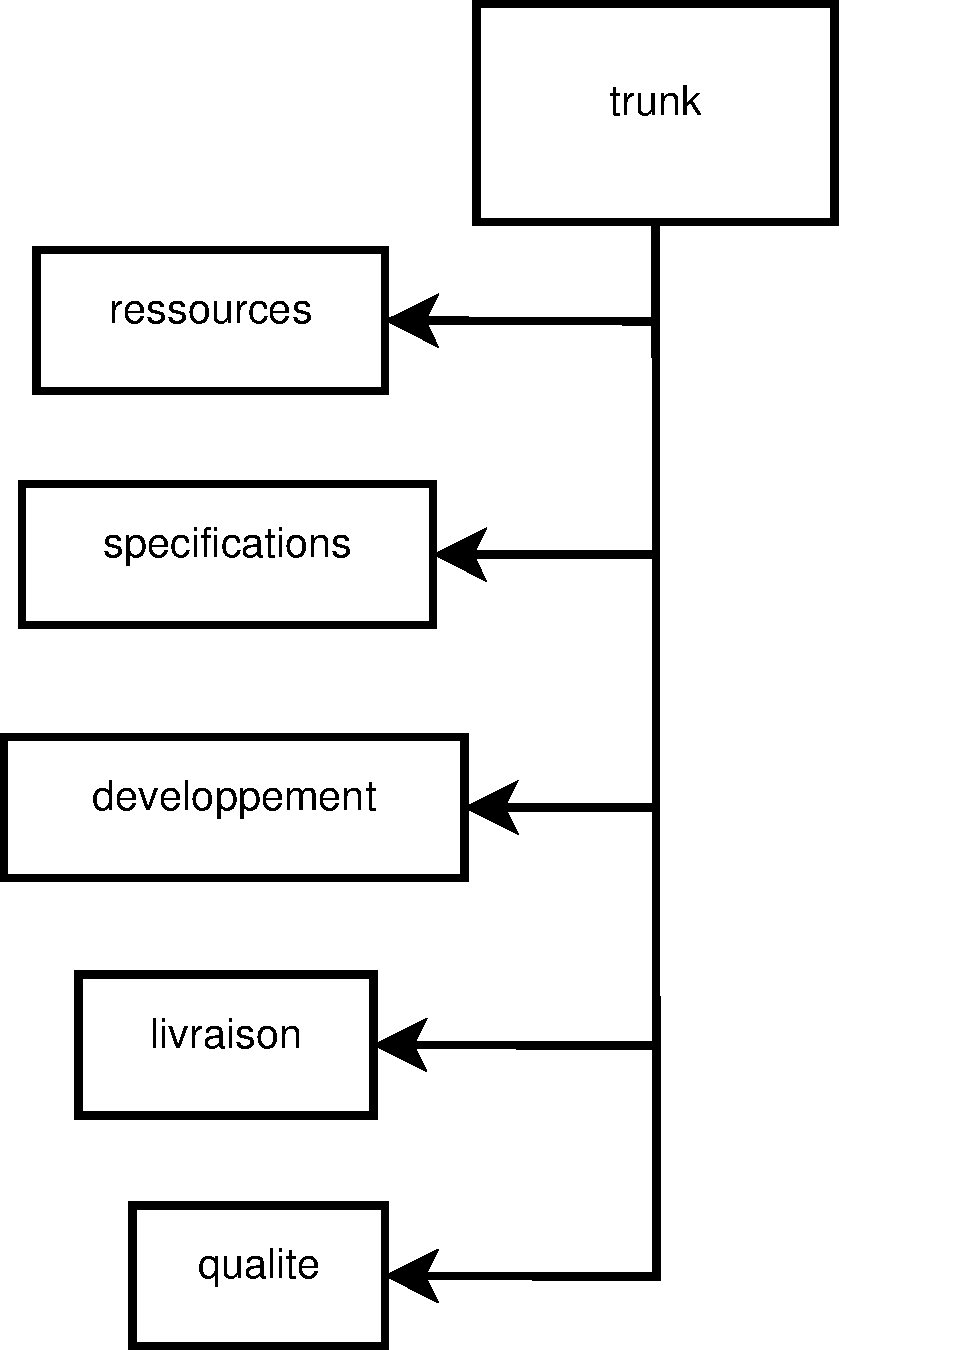
\includegraphics[scale=1.0]{images/arboTrunk}
         \end{center}
         \caption{Structure générale}
 \end{figure}
 
 \section{Référentiel de qualité}
 % version 1.00	Auteur Mathieu Médici

Le référentiel Qualité contient l'ensemble des documents produits par l'équipe \nomEquipe{} dans la cadre de sa démarche qualité.

\begin{figure}[ht]
         \begin{center}
         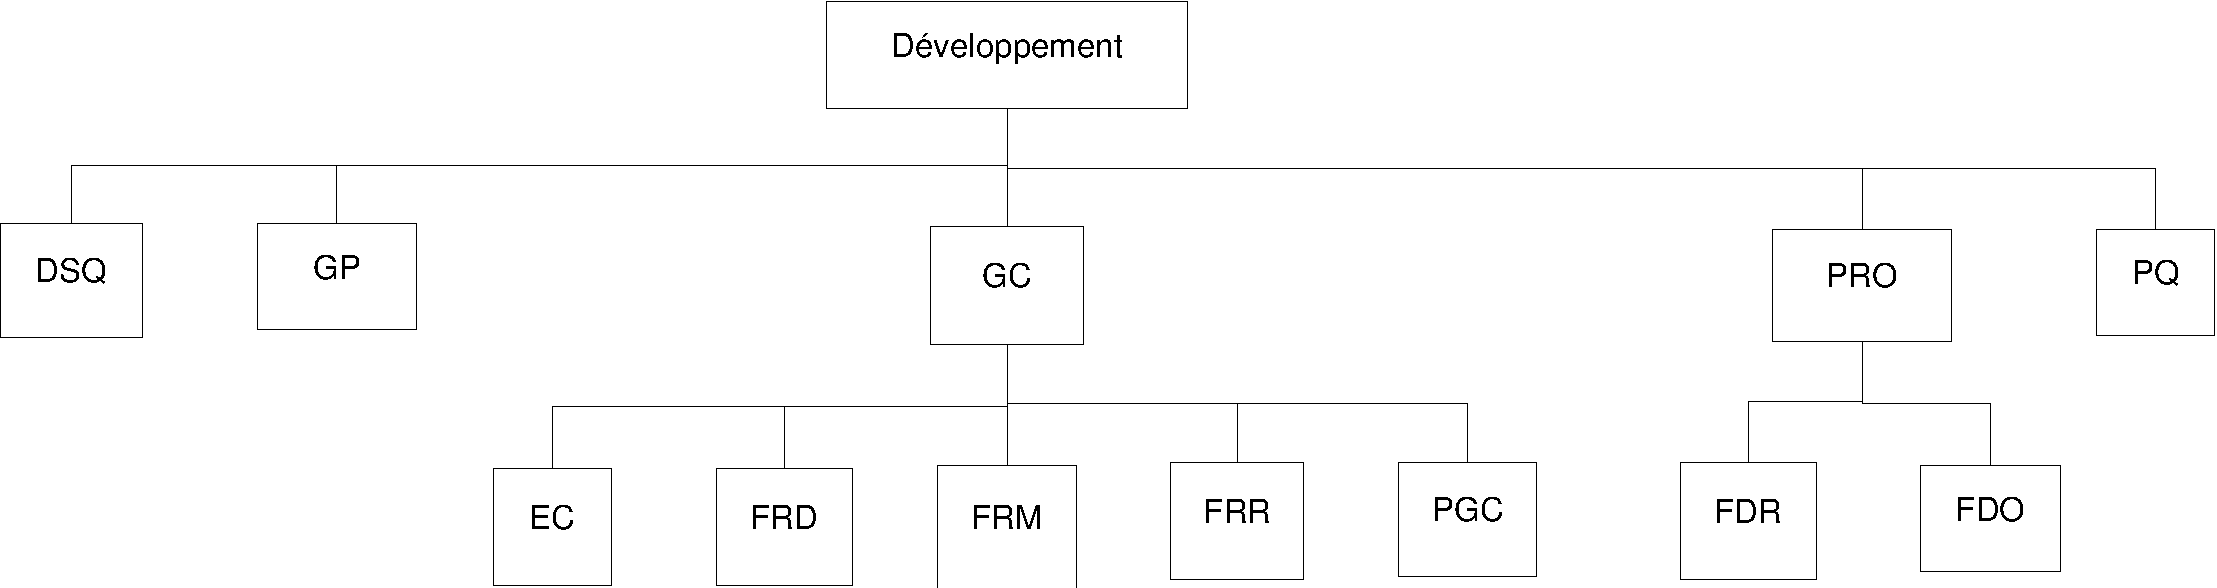
\includegraphics[scale=0.5]{images/arboQualite}
         \end{center}
         \caption{Référentiel Qualité}
 \end{figure}

\clearpage 

\subsection{Structure du répertoire GP}
\addcontentsline{toc}{subsection}{Structure du répertoire GP}

\begin{figure}[ht]
         \begin{center}
         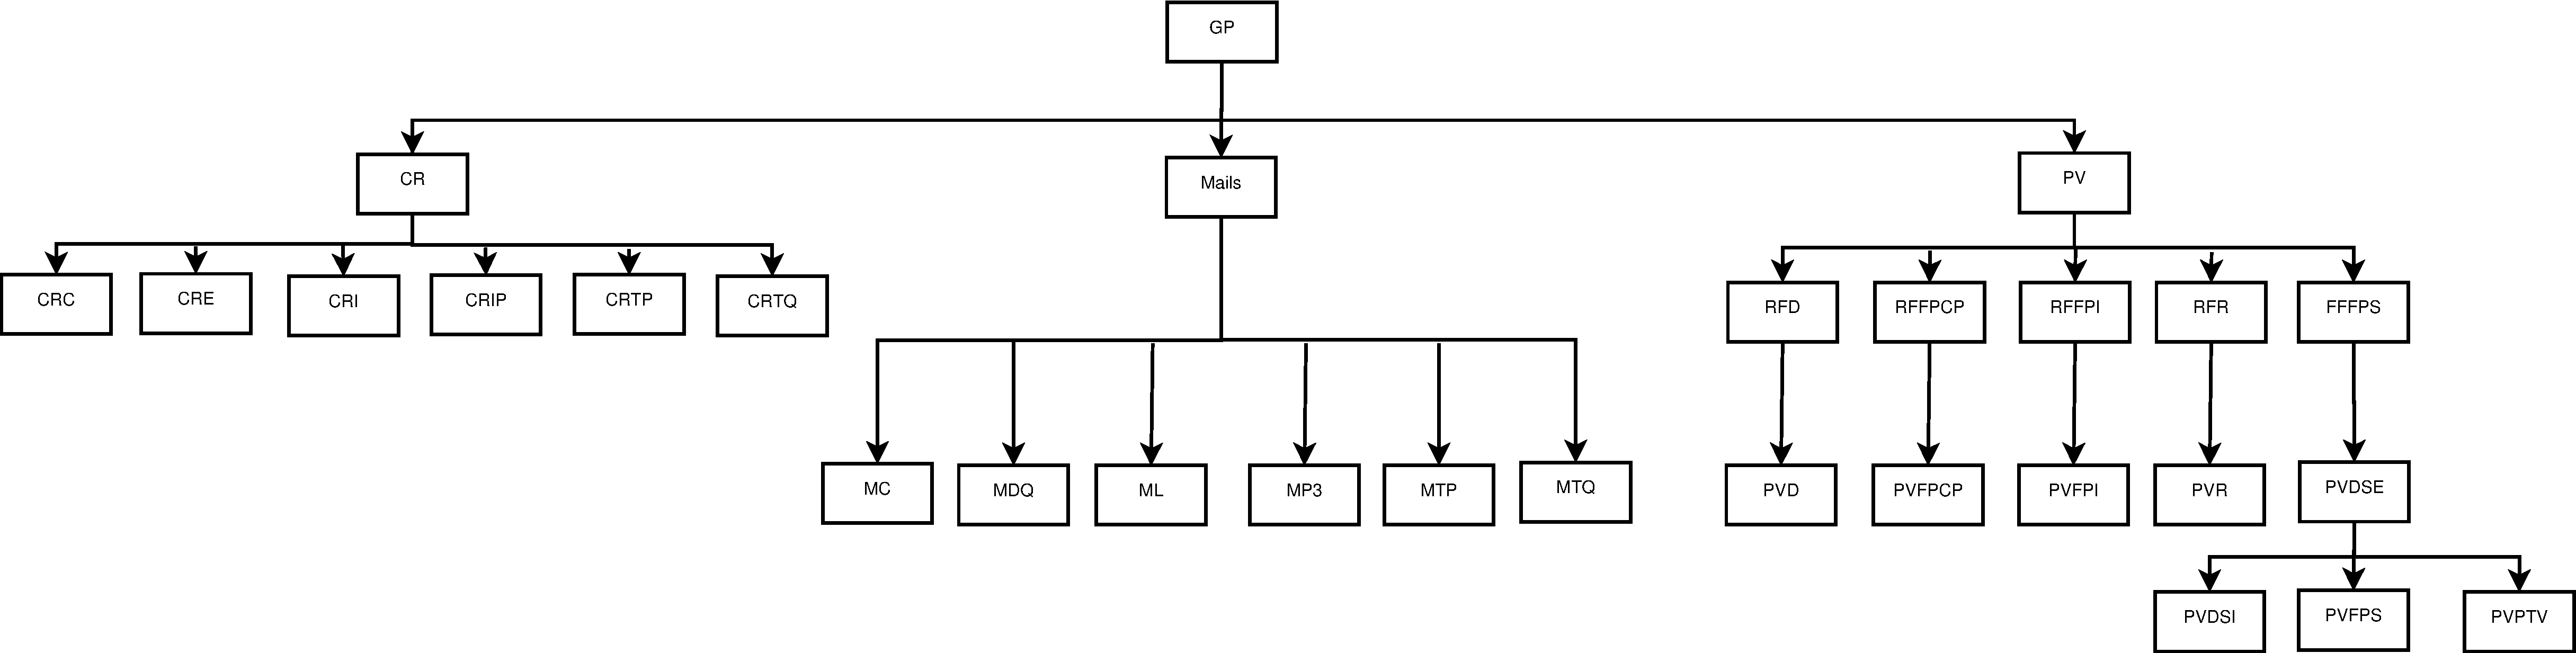
\includegraphics[scale=0.24]{images/arboGP}
         \end{center}
         \caption{Référentiel Qualité - Gestion de Projet}
 \end{figure}
 
 \subsection{Structure du répertoire DSQ}
\addcontentsline{toc}{subsection}{Structure du répertoire DSQ}

\begin{figure}[ht]
         \begin{center}
         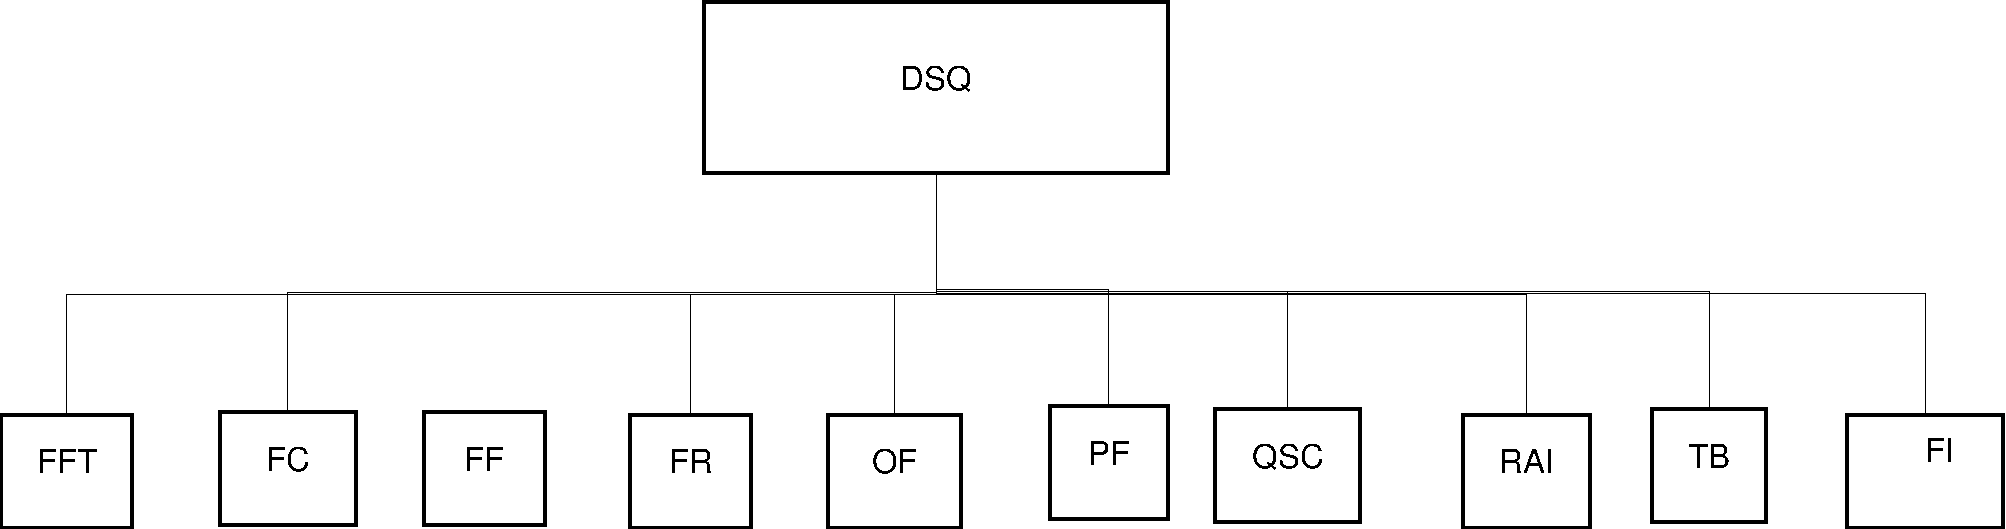
\includegraphics[scale=0.6]{images/arboDSQ}
         \end{center}
         \caption{Référentiel Qualité - Dossier de Suivi de la Qualité}
 \end{figure}


  
 \section{Référentiel de spécifications}
 % version 1.01 Date 14/03/2016	Auteur Mathieu Medici

Le référentiel Spécification contient l’ensemble des documents réalisés pendant la phase de spécification du \PICCourt.

\clearpage

\begin{figure}[ht]
         \begin{center}
         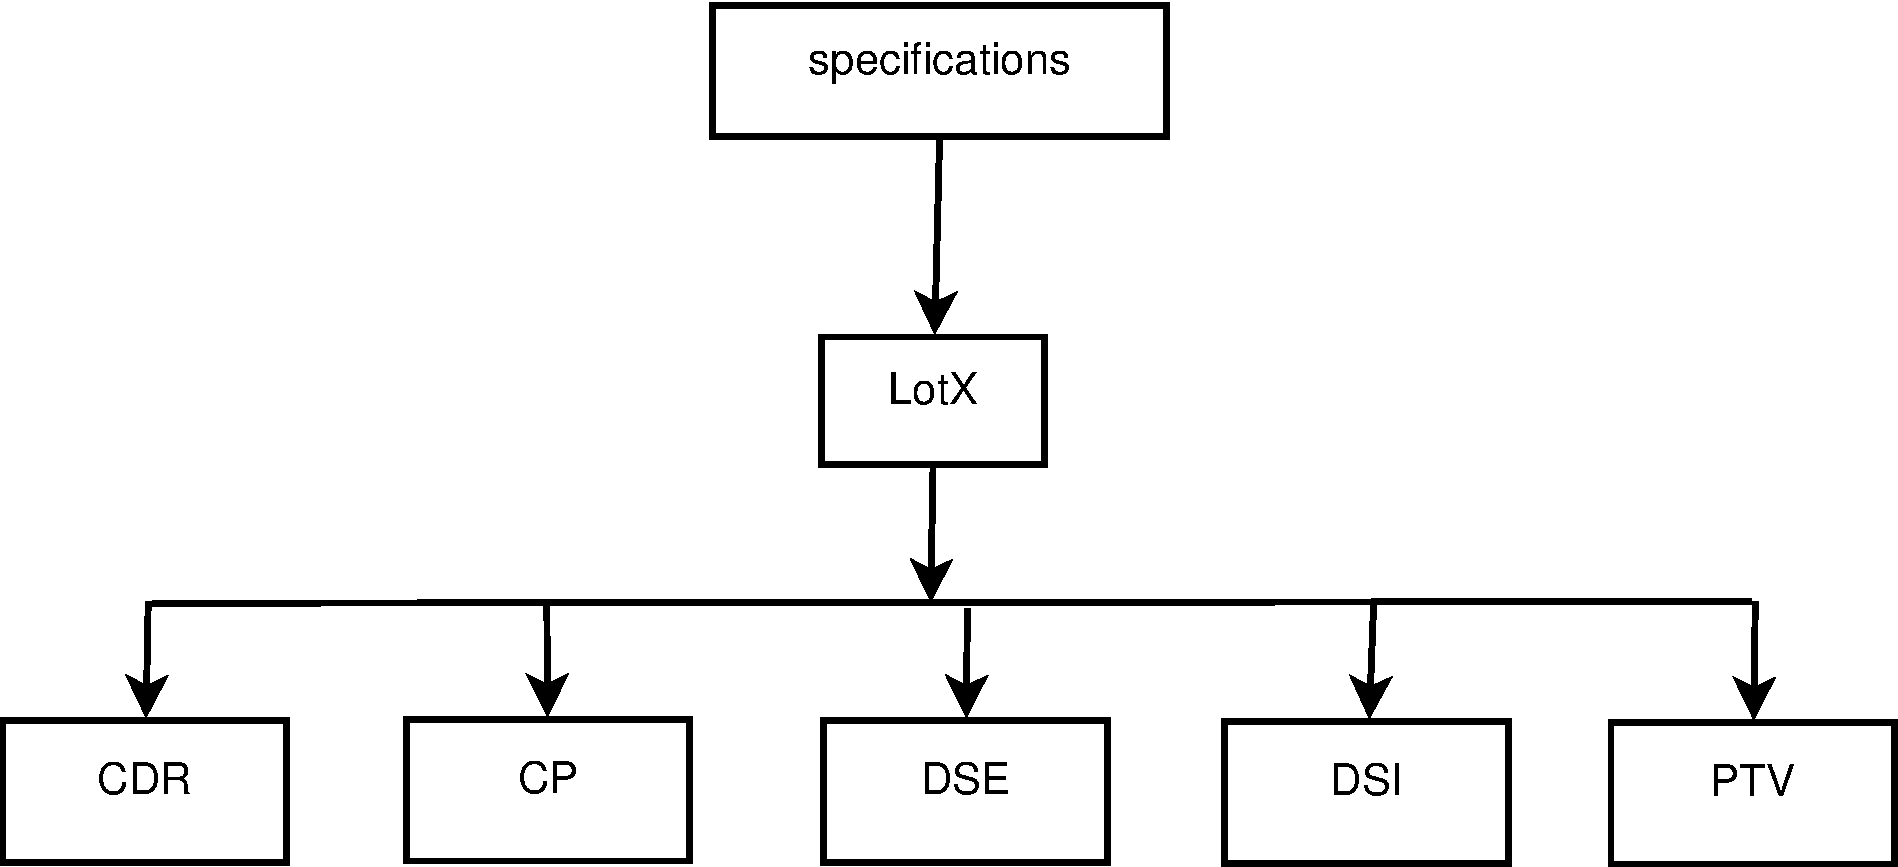
\includegraphics[scale=0.50]{images/arboSpecifications}
         \end{center}
         \caption{Référentiel Spécifications}
 \end{figure}

 
  \section{Référentiel de développement}
 Le référentiel Développement contient l’ensemble des documents réalisés et implémentés au cours du \picCourt.

\clearpage

\begin{figure}[ht]
         \begin{center}
         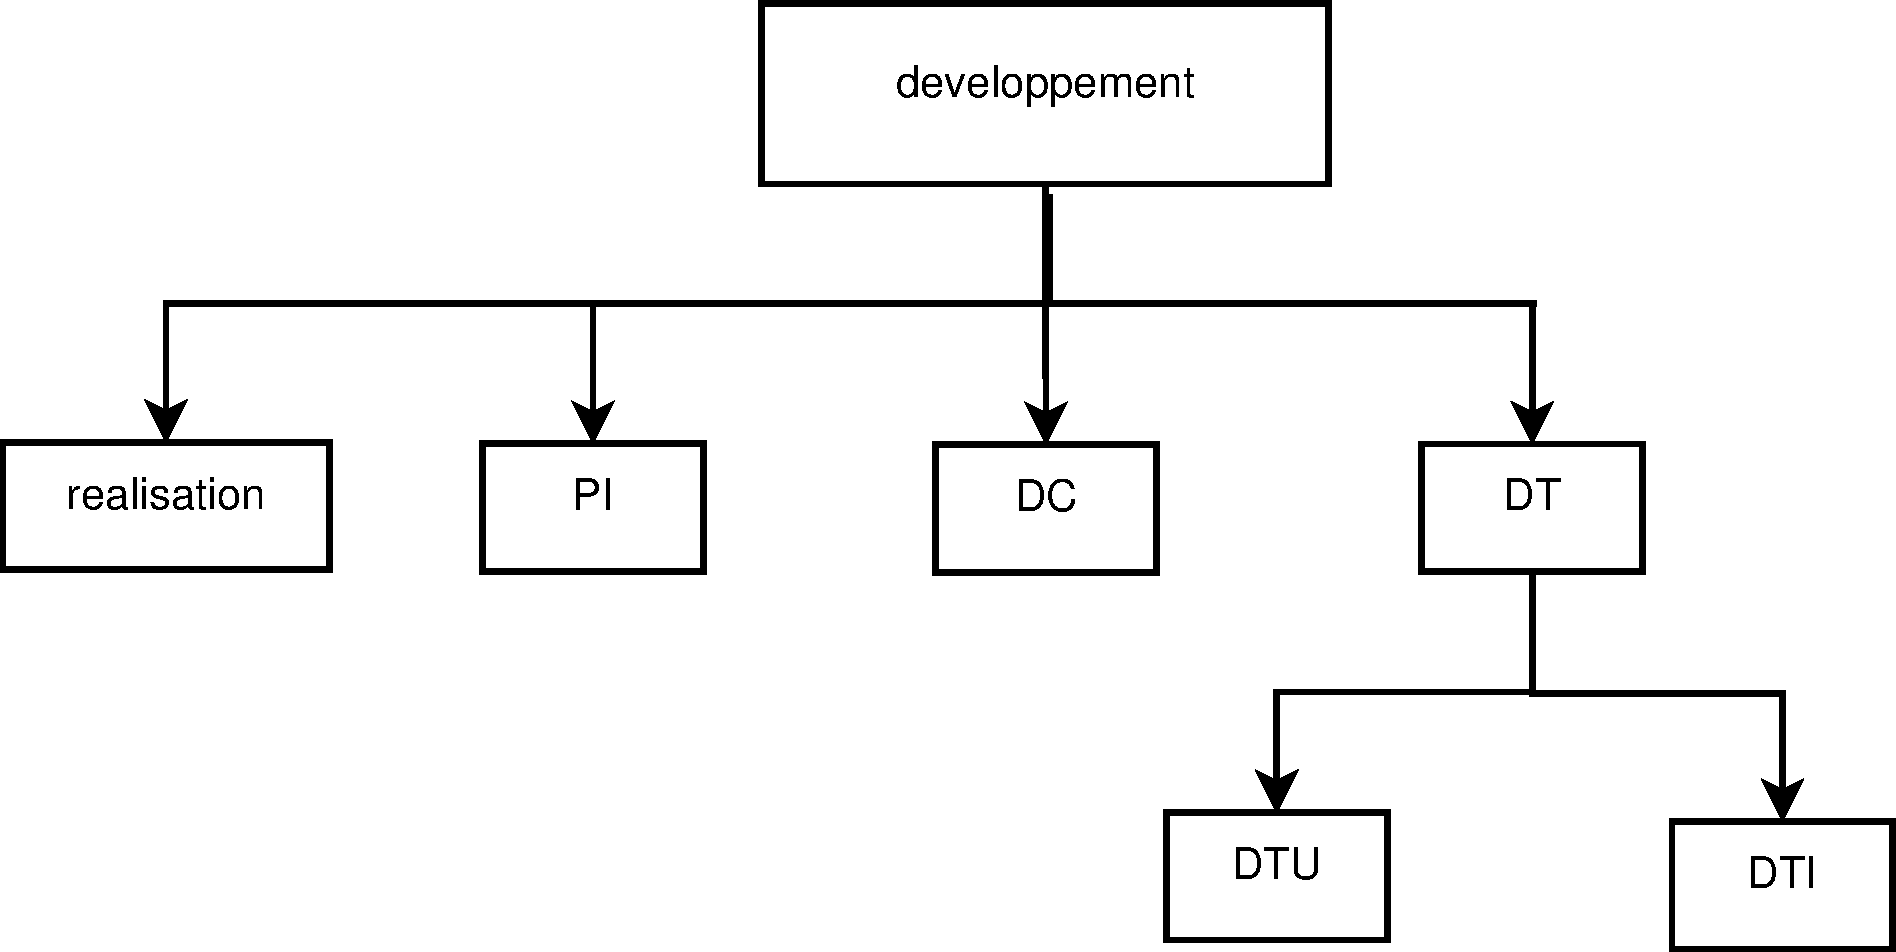
\includegraphics[scale=0.5]{images/arboDeveloppement}
         \end{center}
         \caption{Référentiel Développement}
 \end{figure}

 
  \section{Référentiel de livraison}
 % version 1.01 Date 31/03/2016	Auteur Mathieu Medici

Le référentiel Livraison contient l'ensemble des livrables de \nomEquipe{}.

\clearpage

\begin{figure}[ht]
         \begin{center}
         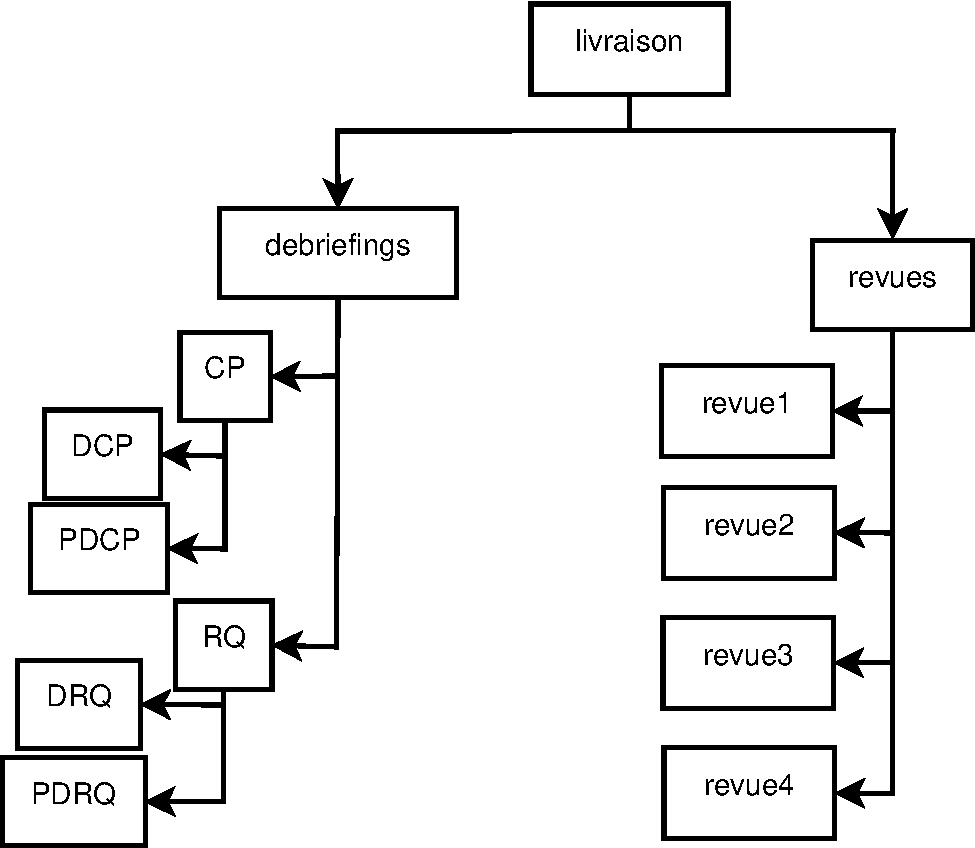
\includegraphics[scale=0.5]{images/arboLivraison}
         \end{center}
         \caption{Référentiel Livraison}
 \end{figure}

%\section{Précisions}


%Le répertoire \textbf{livraisons complémentaires} contient les documents livrés au Client
%en dehors des livraisons officielles des lots. Il se trouve dans le \textbf{FTP}.
%Par exemple, si le Client veut prendre connaissance de notre \planQualite{}, 
%il sera placé dans ce répertoire. 
%Ainsi, ce répertoire permettra le traçage de tout ce qui a été envoyé au client en dehors des livraisons.


%~ Le répertoire \textbf{SP}, placé dans le répertoire \textbf{lots}
%~ correspond au support de présentation dans le cas où il y a une présentation orale
%~ de la part de \nomPIC{} pour le Client.

%Pour le cas où une présentation orale est demandée par le Client, 
%le support de présentation sera placé dans le répertoire \textbf{SP}.

 
  \section{Référentiel de ressources}
 Le référentiel Ressources contient l'ensemble des fichiers et des documents utiles au fonctionnement interne de \nomEquipe{}.

\begin{figure}[ht]
         \begin{center}
         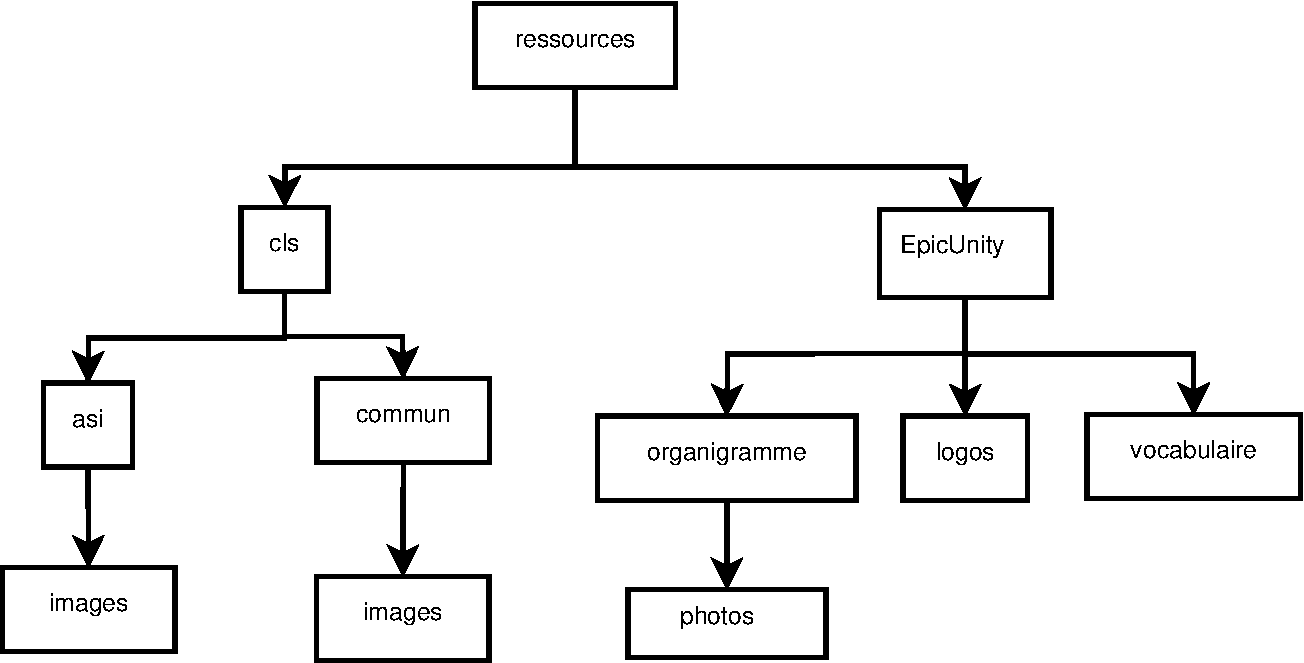
\includegraphics[scale=0.78]{images/arboRessources}
         \end{center}
         \caption{Référentiel Ressources}
 \end{figure}



 \chapter{Règles spécifiques}
 \label{chap regles specifiques}
  % version 1.01 Date 08/03/2016	Auteur Mathieu Medici

\section{Référentiels spécifiques}

Le référentiel \textbf{Ressources} ne sera pas soumis aux conventions de nommage mais certaines règles doivent être respectées. Chaque dossier et chaque fichier devra être nommé en lowerCamelCase et de manière évoquateur quant au contenu. 

\section{Dossiers spécifiques}

\subsection{Dossiers images}

\`{A} la racine du répertoire des documents nécessitant l'inclusion d'images, de diagrammes ou
d'autres figures, se trouve un répertoire \textbf{images}. Il est ajouté au \git{} par le
rédacteur du document si besoin est. Dans ce répertoire sont stockés les fichiers du projet
(\verb+.dia+, \verb+.xcf+, \verb+.jpg+, etc\dots). Les \verb+.pdf+ de ces fichiers sont générés
à la compilation par le \verb+makefile+.
Les fichiers du répertoire \verb+images+ ne sont pas soumis aux conventions de nommage mais certaines règles doivent être respectées. Chaque fichier devra être nommé en lowerCamelCase et de manière évoquateur quant au contenu. 

\subsection{Dossiers sources}

\`{A} la racine du répertoire des documents nécessitant l'inclusion de sous-fichiers \verb+.tex+
(correspondant à des chapitres, des sections, etc\dots) se trouve un répertoire \textbf{sources} pour
les documents longs nécessitant d'être subdivisés. 
Ces sous-fichiers \verb+.tex+ seront placés dans ce répertoire et ils seront inclus via
le \verb+.tex+ général. Ces sous-fichiers ne sont pas soumis aux conventions de nommage mais certaines règles doivent être respectées.\\
Chaque fichier devra être nommé de la manière suivante :
\begin{center}
\verb+<Numéro>_<Nom>+
\end{center}
\begin{itemize} 
\item Numéro : numéro du document variant de \verb+01+ à \verb+99+ et prenant la valeur particulière \verb+00+ pour les pages de services;
\item Nom : nom du document en lowerCamelCase et évocateur quant au contenu.\\
\end{itemize}
Exemples : \\
\verb+00_pageService.tex+\\
\verb+01_introduction.tex+\\
\verb+02_partie1.tex+\\

Remarque : si un fichier source appelle d'autres sources, il faut créer un dossier du même nom que le nom du document et dont les fichiers respectent aussi les règles ci-dessus.\\
Exemple : \\
\verb+\partie1+\\
\hspace*{1cm} \verb+01_sousPartie1.tex+\\
\hspace*{1cm} \verb+02_sousPartie2.tex+\\
\hspace*{1cm} \verb+03_sousPartie3.tex+\\

\subsection{Dossiers annexes}

\`{A} la racine du répertoire des documents nécessitant l'inclusion d'annexes se trouve un répertoire \textbf{annexes}.
Ces documents seront placés dans ce répertoire et ils seront inclus via
le \verb+.tex+ général. Ces sous-fichiers ne sont pas soumis aux conventions de nommage mais certaines règles doivent être respectées. Chaque fichier devra être nommé en lowerCamelCase et de manière évoquateur quant au contenu. 

\subsection{Dossiers pdf}

\`{A} la racine du répertoire de chaque document se trouve un répertoire \textbf{pdf}. C'est
le répertoire dans lequel est placé le \verb+pdf+ généré par la compilation \LaTeX{}. Le \verb+pdf+ n'est pas stocké sur le \git{}.

\subsection{Dossiers enregistrements}

Les dossiers \textbf{enregistrements} permettent de stocker les sources des documents présents dans le répertoire associé à ces documents.\\
Exemple : Le répertoire \verb+pic_unicef/qualite/GP/CR/CRC+ regroupe l'ensemble des Comptes Rendus Client, on y trouve alors un dossier \verb+enregistrements+ qui contient l'ensemble des sources, un dossier \verb+pdf+ pour le stockage sur SA MACHINE des pdf et le makefile qui compile toutes les sources en même temps.


\section{Précisions sur les répertoires de l'arborescence}

\subsection{Répertoire implementation}

Localisation : \verb+pic_unicef/developpement/implementation+\\

Le répertoire implementation est constitué de dossiers représentatifs des différentes applications à produire par le PIC. Le nom de ces dossiers et leur organisation sont gérés par le responsable développement.

\subsection{Répertoire lotX}

Localisations : \\
\verb+pic_unicef/developpement/lotX+\\
\verb+pic_unicef/livraison/lots/lotX+\\

Les répertoires lotX contiendront, en plus des livraisons officielles prévues, le Cahier De Recette du lot concerné annoté par le client.

\subsection{Répertoire client}

Localisation : \verb+pic_unicef/ressources/client+\\

Le répertoire client contient l’ensemble des documents fournis par le client à \nomEquipe.


\section{Règles de rédaction des dates}

Les dates figurant dans les documents sont toutes au format \textbf{JJ/MM/AAAA}. Attention à ne pas confondre avec le format de date des  suffixes dans la convention de nommage (\verb+dAA-MM-JJ+).



 \chapter{Administration des configurations}
  \section{Suivi des configurations}

Afin de permettre le suivi de ces documents ainsi que leur état en temps réel, \nomEquipe{} utilise l'intranet \lintranet. 
Il permet de savoir quelle est la dernière version applicable d'un document et récapitule l'ensemble du contenu des référentiels. 
Cette page est actualisée par la personne concernée lors de la création, la vérification, la validation, l'approbation, la diffusion et l'archivage d'un document. Sur cette page figurent les informations suivantes:
\begin{itemize}
	\item \textbf{référentiel}: nom du référentiel auquel le document appartient;
	\item \textbf{document}: nom du document;
	\item \textbf{rédacteur}: nom du rédacteur qui a initié le document;
	\item \textbf{vérificateur}: nom du vérificateur;
	\item \textbf{validateur}: nom du validateur;
	\item \textbf{approbation}: le document a été approuvé ou non (case verte si le document a été
	approuvé, rouge sinon);
	\item \textbf{diffusion}: le document a été diffusé ou non (case verte si le document a été
	diffusé, rouge sinon);
	\item \textbf{archivage}: le document a été archivé ou non (case verte si le document a été
	archivé, rouge sinon);
	\item \textbf{référence}: nom complet du document;
	\item \textbf{localisation}: où a été diffusé le document;
	\item \textbf{chemin}: chemin complet d'accès au document sur le \git.
\end{itemize}


\section{État de Configuration}
\label{EC}

Un État de configuration décrit l'état des documents demandés par leur destinataire à une date donnée. Un état de configuration doit être généré entre autres à chaque livraison. Ils suivent le modèle présenté en Annexe \ref{modèle EC}. Il doit être composé de tous les documents nécessaire à la livraison : 
\begin{itemize}
\item \textbf{Pour une livraison client:}
	\begin{itemize}
	\item les livrables (code source, procédure d'installation, documentation technique);
	\item les documents de spécification.
	\end{itemize}
\item \textbf{Pour une inspection technique:}
	\begin{itemize}
	\item le code source;
	\item les documents de spécification;
	\item les documents qualité;
	\item les documents de gestion de projet (exemple: comptes-rendus de réunion) nécessaires à la compréhension des autres documents.\\
	\end{itemize}
\end{itemize}


Chaque fiche comprend un tableau indiquant les informations suivantes pour chaque document :
\begin{itemize}
	\item \textbf{Type}: le type du document. \\
	Exemple : \verb+PQ+;
	\item \textbf{Destinataire}: le destinataire du document;
	\item \textbf{Référence du document}: la référence complète du document. \\
	Exemple : \verb+PGC_Q_Unipik_v1.00+;
	\item \textbf{Date de création}: date de création du document.\\
	Format : \verb+JJ/MM/AAAA+ ;
	\item \textbf{Raisons}: le but de l'envoi de ce document.\\
	Exemple : \verb+Livraison lot 1+.
\end{itemize}


\bigskip
Par sa signature, le vérificateur de l'État de Configuration atteste avoir vérifié la présence
de tous les éléments nécessaires à la livraison ainsi que leur cohérence, tant au niveau de
la forme que du fond.

\paragraph{Précision du suffixe :}
Le suffixe de l'état de configuration est de type date et commentaire. Le suffixe \verb+date+ correspond à la date à laquelle les documents ont été envoyés par l’émetteur. Le suffixe \verb+commentaire+ doit définir la raison de la création de l'état de configuration. Les valeurs possibles sont :
\begin{itemize}
\item \verb+Inspection+;
\item \verb+Livraison+;
\item \verb+<NomDoc>+; \\
Exemple : \verb+cPQ+
\item \verb+Autre+.
\end{itemize}
Exemple : \verb+EC_Q_Unipik_d16-03-05_cLivraison+

\section{Fiche d'Etat des Données Client}
\label{FEDC}

Une Fiche d'Etat des Données Client (FEDC) décrit l'ensemble des documents envoyées par le client. Elle suit le modèle présenté en Annexe \ref{modèle FEDC}. Pour chaque document, la FEDC comprend un tableau indiquant les informations suivantes :
\begin{itemize}
\item \textbf{Emetteur} : l'émetteur du document;
\item \textbf{Date} : la date de réception du document (format : \verb+JJ/MM/AAAA+);
\item \textbf{Stockage} : le chemin complet du document (où il est stocké);
\item \textbf{Détruit} : indique si le document a été détruit ou s'il est encore possédé par \nomEquipe. Les valeurs possibles sont \{Oui, Non\};
\item \textbf{Date de destruction} : indique la date de destruction si elle a eu lieu (format : \verb+JJ/MM/AAAA+).
\end{itemize}

\paragraph{Précision sur le suffixe :}
La FEDC ne possède pas de suffixe. En effet il n'y a qu'une seule FEDC qui sera mise à jour au fur et à mesure que nous recevons de nouvelles données ou que des données sont déplacées ou supprimées.

 \chapter{Maîtrise des documents}
  \section{Historique des évolutions}

Les modifications apportées à un document apparaissent dans sa page de service. À chaque modification il faut indiquer les informations suivantes :
\begin{itemize}
 \item \textbf{version}: indique le numéro de version du document suite à la modification apportée;
\item \textbf{date} : indique la date de la dernière modification du document dans le format \verb+JJ/MM/AAAA+;
\item \textbf{auteur} : indique les noms complets des personnes ayant effectué les modifications;
\item \textbf{modification} : décrit brièvement le type de modification apportée. Si le document a
été diffusé, cette section comprend obligatoirement :
	\subitem \textbullet{ }le numéro de la Fiche d'\OC{} (FOC) qui a donné lieu à la modification;
	\subitem \textbullet{ }le numéro de la Fiche de Fait Technique (\FFTCourt{}) qui lui est associée.
\item \textbf{parties modifiées} : indique les numéros de chapitres et de sections modifiés.
\end{itemize}

\section{Suivi des diffusions}

Le suivi des diffusions est indiqué dans la page de service du document. Il comprend trois informations pour chaque diffusion :
\begin{itemize}
\item \textbf{version} : indique la version du document concerné par la diffusion ;
\item  \textbf{date} : indique la date de diffusion de document ;
\item \textbf{destinataire} : indique les destinataires du document. 
\end{itemize}
 Le suivi des diffusions n’est rempli qu’une fois le document approuvé.

\section{Signatures}

Le contrôle de la vérification, de la validation et de l’approbation d’un document est visible dans la page de service. Il comporte trois lignes correspondant aux trois personnes en charge de ces étapes. Les trois personnes doivent être différentes. L'auteur du document ne peut pas en faire partie.\\

Le \textbf{vérificateur} est responsable de la relecture du document afin d’en vérifier l’orthographe et la cohérence du contenu. Il ne peut en aucun cas être l'auteur du document vérifié..\\

Le \textbf{validateur} évalue la pertinence du document après qu’il ait été vérifié, il engage aussi sa responsabilité en ce qui concerne la correction du document. Il est en charge de la diffusion du document vers les destinaires identifiés et de la mise à jour des dossiers \verb+approbations+.\\

L’\textbf{approbateur} est une personne externe au \pic{}, en charge de l’acceptation du document.

Pour chacune des trois étapes doivent apparaître les informations suivantes dans la page de service :
\begin{itemize}
\item \textbf{fonction} : la fonction de la personne ayant effectué l’étape ;
\item  \textbf{nom} : le nom de la personne ayant effectué l’étape ;
\item \textbf{date} : la date où l’étape a été effectuée ;
\item \textbf{visa} : la mention "signé" est ajoutée aux documents électroniques, une fois le document signé numériquement. La signature numérique doit être archivée, c'est le seul document permettant de certifier de la signature du document.

\end{itemize}



\chapter{Maîtrise des enregistrements}
 % version 1.01 Date 08/03/2016	Auteur Mathieu Medici

\section{Définition des enregistrements}

Tous les enregistrements exigés par la norme \isoNeufMilleUn{} sont enregistrés dans le dépôt \git. Ils doivent rester lisibles, identifiables et accessibles à tout moment.

\section{Maîtrise des évolutions}

Les enregistrements nous permettent de suivre l’évolution des configurations. L’évolution des enregistrements est soumise aux règles suivantes :
\begin{itemize}
\item aucune modification ou évolution non autorisée sur un document ne peut être effectuée ;
\item la restitution d’un enregistrement doit être possible à tout instant.
\end{itemize}

Pour respecter ces règles, un dossier \textbf{approbations}, contenant les preuves de l’approbation du document, sera placé dans le dossier de base du document.\\



 \chapter{Archivage}
  \label{archivages}
  % version 1.01 Date 08/03/2016	Auteur Mathieu Medici

Ce chapitre présente comment les documents, versionnés ou non, seront archivés dans le cadre de notre projet. L’archivage se divise en deux parties : l’archivage informatique et l’archivage papier.

\section{Archivage informatique}
L'archivage informatique se divise en trois parties : le stockage du projet sur le serveur \git{}, l'archivage sur PGPic et le stockage des documents approuvés.

\subsection{Stockage du projet sur \git{}}
Tous les documents courants du \PICCourt sont stockés de façon numérique sur le serveur \git{} mis à disposition par le département \ASI{}. On y trouve à la fois les documents relatifs à la démarche qualité, mais aussi le code, les mails, ou tout autre document créé pour le projet.

\subsection{Archivage sur le serveur PGPic}

Chaque semaine, le \RQ{} procède à un archivage des documents au format \verb+pdf+. Cette archivage sera stockée sur notre compte du serveur PGPic.

\subsection{Stockage des documents approuvés}



\section{Archivage papier}
Certains documents nécessitent un archivage papier spécifique car ils comportent pour la plupart des signatures manuscrites. Ils sont obligatoirement rangés dans le classeur correspondant se trouvant dans l’armoire de la salle du projet. Ces documents sont :
\begin{itemize}
\item Engagements de confidentialité;
\item Rapports d’audits;
\item Formations;
\item Procès verbaux.
\end{itemize}
Ces documents ne doivent pas sortir de la salle.


 \begin{appendix}
	\part*{Annexes}
	\addcontentsline{toc}{part}{Annexes}
	\chapter{Modèle de l'État de configuration}
	% version 1.00	Auteur Mathieu Médici

\label{modèle EC}

\begin{center}
\huge
\nomEquipe{}\\
État de Configuration\\
\end{center}
\vspace{0.5cm}


\begin{figure}[H]
		\centering
		\begin{tabularx}{17cm}{|p{4cm}|X|X|}
		\hline
		\rowcolor[gray]{0.85}Date de création & Destinataire & Raisons \\
		\hline
		 &  & \\
		\hline
		\end{tabularx}
\end{figure}

\subsection*{Liste de documents}

\begin{figure}[H]
		\centering
		\begin{tabularx}{17cm}{|p{7cm}|X|}
		\hline
		\rowcolor[gray]{0.85}Type & Référence du document\\
		\hline
		\multicolumn{2}{|c|}{\textit{Référentiel Qualité}}\\
		\hline 
		  &   \\
		 \hline 
		\multicolumn{2}{|c|}{\textit{Référentiel Développement}}\\
		\hline 
		 &   \\
		\hline 
		\multicolumn{2}{|c|}{\textit{Référentiel Spécification}}\\
		\hline
		& \\
		\hline 
		\multicolumn{2}{|c|}{\textit{Référentiel Livraison}}\\
		\hline
		& \\
		\hline 
		\end{tabularx}
\end{figure}

\subsection*{Signature}

\begin{figure}[H]
		\centering
		\begin{tabularx}{17cm}{|p{4cm}|X|X|X|X|}
		\hline
		\rowcolor[gray]{0.85}& Fonction & Nom & Date & Visa \\
		\hline
		 Vérificateur de l'EC &  & & &  \\
		\hline
		\end{tabularx}
\end{figure}

	\chapter{Modèle de la Fiche d'Etat des Données Client}
	% version 1.00	Auteur Mathieu Médici

\label{modèle FEDC}

\begin{center}
\huge
\nomEquipe{}\\
Fiche d'Etat des Données Client\\
\end{center}
\vspace{0.5cm}


\begin{longtable}{|p{2cm}|p{2.2cm}|p{6cm}|p{2cm}|p{2.4cm}|}
    \hline
    \rowcolor[gray]{0.55}\multicolumn{5}{|c|}{\textbf{\bsc{Nom Document 1}}}\\
    \hline
    \rowcolor[gray]{0.85} \centering{Emetteur} & \centering{Date} & \centering{Stockage} & \centering{Détruit} & Date de destruction\\
    \hline
     &  &  &  &  \\
    \hline 
\end{longtable}

\begin{longtable}{|p{2cm}|p{2.2cm}|p{6cm}|p{2cm}|p{2.4cm}|}
    \hline
    \rowcolor[gray]{0.55}\multicolumn{5}{|c|}{\textbf{\bsc{Nom Document 2}}}\\
    \hline
    \rowcolor[gray]{0.85} \centering{Emetteur} & \centering{Date} & \centering{Stockage} & \centering{Détruit} & Date de destruction\\
    \hline
     &  &  &  &  \\
    \hline 
\end{longtable}
	\listoffigures
	 \addcontentsline{toc}{chapter}{Liste des figures}
	 
	\listoftables
	 \addcontentsline{toc}{chapter}{Liste des tableaux}
 \end{appendix}

\newpage

\pageQuatriemeCouverture{}

\end{document}
